\textbf{Метод 4 --- Метод Стрельбы/Метод конечных разностей}\\

\textbf{Задание}

Реализовать метод стрельбы и конечно--разностный метод решения краевой задачи для ОДУ в виде программ. С использованием разработанного программного обеспечения решить краевую задачу для обыкновенного дифференциального уравнения 2--го порядка на указанном отрезке. Оценить погрешность численного решения с использованием метода Рунге-Ромберга и путем сравнения с точным решением.\\

\textbf{Вариант:} 3

Краевая задача:

$x^2(x+1)y''-2y=0$\\
$y'(1)=-1$\\
$2y(2)-4'(2)=4$\\

Точное решение:

$y(x)=\frac{1}{x}+1$\\

\textbf{Описание алгоритма}

Примером краевой задачи является двухточечная краевая задача для обыкновенного дифференциального уравнения второго порядка.\\

$y''=f(x, y, y')$\\

с граничными условиями первого порядка, заданными на концах отрезка $[a, b]$.\\

$y(a)=y_0$\\
$y(b)=y_1$\\

Следует найти такое решение $y(x)$ на этом отрезке, которое принимает на концах отрезка значения $y_0, y_1$. Если функция $f(x, y, y')$ линейна по аргументам $y, y'$, то задача является линейной краевой задачей, в противном случае --- нелинейной.\\

Граничные условия второго порядка:\\

$y'(a)=\hat{y_0}$\\
$y'(b)=\hat{y_1}$\\

Граничные условия третьего порядка:\\

$\alpha y(a) + \beta y'(a) = \hat{y_0}$\\
$\delta y(b) + \gamma y'(b) = \hat{y_1}$\\

где $\alpha, \beta, \delta, \gamma$ --- такие, что $|\alpha|+|\beta| \neq 0, |\delta|+|\gamma| \neq 0$\\

Возможно на разных концах отрезка использовать условия различных типов.\\

\textbf{Метод стрельбы}\\

Суть метода заключается в многократном решении задачи Коши для приближенного нахождения решения краевой задачи.\\

В случае $\beta \neq 0$ задается $y(a)=\eta$, а $y'(a)=\frac{\hat{y_0}-\alpha \eta}{\beta}$.\\
В случае $\beta = 0$ задается $y'(a)=\eta$, а $y(a)=\frac{\hat{y_0}}{\alpha}$\\

В данном случае $\eta$ --- некоторое значение либо высоты, либо угла наклона, которое нужно найти.

При использовании метода деления пополам или метода секущих берутся произвольные $\eta_0, \eta_1$ такие, чтобы значения функций $\Phi(\eta_0), \Phi(\eta_1)$ отличались по знаку.

Другими словами решение исходной задачи эквивалентно нахождению корня уравнения:\\

$\Phi(\eta)=0$ \qquad (1)

где $\Phi(\eta)=y(b, y_0, \eta)-y_1$\\

Уравнение (1) является алгоритмическим уравнением, т.к. левая часть его задается с помощью алгоритма численного решения соответствующей задачи Коши. Следующее значение искомого корня определяется по соотношению:\\

$\eta_{j+2}=\eta_{j+1}-\frac{\eta_{j+1}-\eta_j}{\Phi(\eta_{j+1})-\Phi(\eta_j)}\Phi(\eta_{j+1})$\\

Условие окончания итераций:\\

$|\eta_{j+1}-\eta_{j}| \leq \varepsilon$\\

\textbf{Метод конечных разностей}\\

Рассмотрим двухточечную краевую задачу для линейного дифференциального уравнения второго порядка на отрезке $[a, b]$\\

$y''+p(x)y'+q(x)y=f(x)$\\
$y(a)=y_0, y(b)=y_1$\\

Введем разностную сетку на отрезке $[a, b] \quad \Omega^{(h)}={x_k=x_0+hk}, k=0,1,...,N, h=|b-a|/N$. 

Решение задачи будем искать в виде сеточной функции $y^{(k)}={y_k, k=0,1,...,N}$, предлагая, что решение существует и единственно. Введем разностную аппроксимацию производных следующим образом:\\

$y'_k=\frac{y_{k+1}-y_{k-1}}{2h}+O(h^2)$\\

$y''_k=\frac{y_{k+1}-2y_k+y_{k-1}}{h^2}+O(h^2)$\\

Подставляя аппроксимации производных получим систему уравнений для нахождения $y_k$:

$$
\begin{cases}
(\alpha - \frac{\beta}{h})y_0+(\frac{\beta}{h})y_1=\hat{y_0}\\
(\frac{1}{h^2}-\frac{p(x_k)}{2h})y_{k-1}+(-\frac{2}{h^2}+q(x_k))y_k+(\frac{1}{h^2}+\frac{p(x_k)}{2h})y_{k+1}=f(x_k), k=1,...,N-1\\
(-\frac{\gamma}{h})y_{N-1}+(\delta+\frac{\gamma}{h})y_{N}=\hat{y_1}
\end{cases}
$$

Для системы при достаточно малых шагах сетки $h$ и $q(x)<0$ выполнены условия преобладания диагональных элементов\\

$|-2+h^2q(x_k)|>|1-\frac{p(x_k)h}{2}|+|1+\frac{p(x_k)h}{2}|$\\

что гарантирует устойчивость счета и корректность применения метода прогонки для решения этой системы.

В случае использования граничных условий второго и третьего рода аппроксимация производных проводится с помощью односторонних разностей первого и второго порядков.\\

$y'_0=\frac{y_1-y_0}{h}+O(h)$\\

$y'_N=\frac{y_N-y_{N-1}}{h}+O(h)$ \qquad (1)\\ 

$y''_0=\frac{-3y_0+4y_1-y_2}{2h}+O(h^2)$\\

$y''_N=\frac{y_{N-2}-4y_{N-1}+3y_N}{2h}+O(h^2)$ \qquad (2)\\

В случае использования формул (1) линейная алгебраическая система аппроксимирует дифференциальную задачу в целом только с первым порядком (из-за аппроксимации в граничных точках), однако сохраняется трехдиагональная структура матрицы коэффициентов. В случае использования формул (2) второй порядок аппроксимации сохраняется везде, но матрица линейной системы не трехдиагональная.\\

\textbf{Реализация}\\

\begin{lstlisting}
#include <iostream>
#include <functional>
#include <vector>
#include <utility>
#include <cmath>
#include <fstream>
#include "dependences/TSolve.h"

using namespace std;

// TODO: write method Runge-Romberg

pair<double, double> ToSolveRungeKutta(double a,
									   double b,
									   double h,
									   double funcY0,
									   double funcZ0,
									   function<double(double, double)> FuncExpression,
									   const char* fName) {
	/* Runge-Kutta method */	
	bool flag = false;
	ofstream out;
	if (!!fName) {
		flag = true;
		out.open(fName, ios::out | ios::app);
	}
	vector<double> X, Y, Z;
	double x0 = a, y0 = funcY0, z0 = funcZ0;
	size_t N = (b - a) / h;
	double K1, K2, K3, K4, L1, L2, L3, L4;
	double y_k = y0;
	double x_k = x0;
	double z_k = z0;
	double deltaZ, deltaY;
	for (size_t k = 0; k < N; ++k) {
		L1 = h * FuncExpression(x_k, y_k);
		K1 = h * z_k;		

		K2 = h * (z_k + 0.5 * L1);
		L2 = h * FuncExpression(x_k + 0.5 * h, y_k + 0.5 * K1);

		K3 = h * (z_k + 0.5 * L2);
		L3 = h * FuncExpression(x_k + 0.5 * h, y_k + 0.5 * K2);

		K4 = h * (z_k + L3);
		L4 = h * FuncExpression(x_k + h, y_k + K3);

		deltaY = 1.0 / 6.0 * (K1 + 2.0 * K2 + 2.0 * K3 + K4);
		deltaZ = 1.0 / 6.0 * (L1 + 2.0 * L2 + 2.0 * L3 + L4);

		X.push_back(x_k);
		Y.push_back(y_k);
		Z.push_back(z_k);

		x_k += h;
		z_k += deltaZ;
		y_k += deltaY;		
	}	
	X.push_back(x_k);
	Y.push_back(y_k);
	Z.push_back(z_k);
	if (flag) {
		auto FuncY = [](double x) -> double {
			return 1.0 / x + 1.0;
		};
		vector <double> tmp;
		out.precision(5);
		out << "x : ";
		for (size_t i = 0; i < X.size(); ++i) {
			out << fixed << X[i] << "\t";
			tmp.push_back(FuncY(X[i]));
		}
		out << endl;
		out << "y : ";
		for (size_t i = 0; i < Y.size(); ++i) {
			out << fixed << Y[i] << "\t";
		}
		out << endl;	
		out << "y*: ";
		for (size_t i = 0; i < Y.size(); ++i) {
			out << fixed << tmp[i] << "\t";
		}
		out << endl;			
		out.close();
	}
	return make_pair(Y.back(), Z.back());
}

void ShooterMethod(const char* f) {
	double a = 1.0, b = 2.0, h = 0.1;
	double n1 = b, n2 = b - h, n;
	double eps = 0.0001;
	double funcZ0 = -1.0;
	size_t j = 0;
	bool flag = false;
	vector<double> X, Y;
	auto FuncExpression = [](double x, double y) -> double {
		return 2.0 * y / (x * x * (x + 1.0));
	};
	auto calc = [](double y, double dy) -> double {
		return 2.0 * y - 4.0 * dy;
	};
	auto calcFi = [&calc](const pair<double, double>& p) -> double {
		return calc(p.first, p.second) - 4.0;
	};
	auto checkRightBorder = [&calcFi](const pair<double, double>& p, double eps) -> bool {
		return fabs(calcFi(p)) < eps;
	};

	string fn = f;
	fn += "ShooterMethod";
	ofstream out(fn, ios::out);
	out.precision(5);
	
	out << "\tn\ty\tFi" << endl;
	for (; !flag; j += 2) {
		auto tmp1 = ToSolveRungeKutta(a, b, h, n1, funcZ0, FuncExpression, NULL);
		auto tmp2 = ToSolveRungeKutta(a, b, h, n2, funcZ0, FuncExpression, NULL);			
		out << fixed << j << "\t" << n1 << "\t" << tmp1.first << "\t" << calcFi(tmp1) << endl;
		out << fixed << j + 1 << "\t" << n2 << "\t" << tmp2.first << "\t" << calcFi(tmp2) << endl;
		n = n2 - (n2 - n1) 
			/ (calcFi(tmp2) 
				- calcFi(tmp1)) 
			* calcFi(tmp2);
		n1 = n2;
		n2 = n;			
		auto tmp3 = ToSolveRungeKutta(a, b, h, n, funcZ0, FuncExpression, NULL);
		flag = checkRightBorder(tmp3, eps);
	}
	auto tmp = ToSolveRungeKutta(a, b, h, n2, funcZ0, FuncExpression, NULL);
	out << fixed << j << "\t" << n2 << "\t" << tmp.first << "\t" << calcFi(tmp) << endl;
	out.close();
	ToSolveRungeKutta(a, b, h, n2, funcZ0, FuncExpression, fn.c_str());		
}

void FiniteDifferenceMethod (const char* f) {
	double a = 1.0, b = 2.0, h = 0.1, ya, yb;
	size_t N = fabs(b - a) / h;
	vector<double> X, Y;	
	for (size_t i = 0; i <= N; ++i) {
		X.push_back(a + h * i);
	}
	auto qx = [](double x) -> double {
		return -2.0 / (x * x * (x + 1.0));
	};
	auto funcY = [](double x) -> double {
		return 1.0 / x + 1;
	};

	string fn = f;	
	string inFile = "dependences/inputData"; 
	string outFile = "dependences/outputData";

	ofstream out(fn + "FiniteDifferenceMethod", ios::out);
	ofstream output(outFile, ios::out);
	
	output << N - 1 << endl;
	output << -1.0 + h * h * qx(X[0]) << " " << 1.0 << " " << 0.0 << " " << -h << endl;
	for (size_t i = 1; i < N - 2; ++i) {
		output << 1.0 << " " << -2.0 + h * h * qx(X[i]) << " " << 1.0 << " " << 0.0 << endl;
	}
	output << 1.0 << " " << -2.0 + h * h * qx(X[N - 1]) - 4.0 / (2.0 * h - 4.0) << " " << 0.0 << " " << -4.0 * h / (2.0 * h - 4.0) << endl; 
	output.close();
	
	TSolve solution(outFile, inFile);
	if (!!solution.ToSolveByTripleDiagMatrix()) {
		cerr << "Error: Troubles with method TripleDiagMatrix!" << endl;
		exit(-1);
	}	
	
	ifstream in(inFile, ios::in);
	double temp;
	while (in >> temp) {
		Y.push_back(temp);
	}
	in.close();
	ya = Y[0] + h;
	yb = 4.0 * (h - Y.back()) / (2.0 * h - 4.0);
	out << "\tx\ty\ty*" << endl;
	out.precision(5);
	out << fixed << 0 << "\t" << X[0] << "\t" << ya << "\t" << funcY(X[0]) << endl;
	for (size_t i = 0; i < Y.size(); ++i) {
		out << fixed << i + 1 << "\t" << X[i + 1] << "\t" << Y[i] << "\t" << funcY(X[i + 1]) << endl;
	}
	out << fixed << N << "\t" << X[N] << "\t" << yb << "\t" << funcY(X[N]) << endl;
	out.close();
	output.close();
}

pair<double, double> tempSolutionRK(double a,
								    double b,
								    double h,
								    double funcY0,
								    double funcZ0,
								    function<double(double, double)> FuncExpression,
								    vector<double>* v) {
	/* Runge-Kutta method */	
	bool flag = false;
	if (!!v) {
		flag = true;
	}
	vector<double> X, Y, Z;
	double x0 = a, y0 = funcY0, z0 = funcZ0;
	size_t N = (b - a) / h;
	double K1, K2, K3, K4, L1, L2, L3, L4;
	double y_k = y0;
	double x_k = x0;
	double z_k = z0;
	double deltaZ, deltaY;
	for (size_t k = 0; k < N; ++k) {
		L1 = h * FuncExpression(x_k, y_k);
		K1 = h * z_k;		

		K2 = h * (z_k + 0.5 * L1);
		L2 = h * FuncExpression(x_k + 0.5 * h, y_k + 0.5 * K1);

		K3 = h * (z_k + 0.5 * L2);
		L3 = h * FuncExpression(x_k + 0.5 * h, y_k + 0.5 * K2);

		K4 = h * (z_k + L3);
		L4 = h * FuncExpression(x_k + h, y_k + K3);

		deltaY = 1.0 / 6.0 * (K1 + 2.0 * K2 + 2.0 * K3 + K4);
		deltaZ = 1.0 / 6.0 * (L1 + 2.0 * L2 + 2.0 * L3 + L4);

		X.push_back(x_k);
		Y.push_back(y_k);
		Z.push_back(z_k);

		x_k += h;
		z_k += deltaZ;
		y_k += deltaY;		
	}	
	X.push_back(x_k);
	Y.push_back(y_k);
	Z.push_back(z_k);
	if (flag) {
		for (size_t i = 0; i < Y.size(); ++i) {
			v->push_back(Y[i]);
		}
	}
	return make_pair(Y.back(), Z.back());
}


vector<double> RungeRombergForShooterMethod(double step) {
	double a = 1.0, b = 2.0, h = step;
	double n1 = b, n2 = b - h, n;
	double eps = 0.0001;
	double funcZ0 = -1.0;
	size_t j = 0;
	bool flag = false;
	vector<double> X, Y;
	auto FuncExpression = [](double x, double y) -> double {
		return 2.0 * y / (x * x * (x + 1.0));
	};
	auto calc = [](double y, double dy) -> double {
		return 2.0 * y - 4.0 * dy;
	};
	auto calcFi = [&calc](const pair<double, double>& p) -> double {
		return calc(p.first, p.second) - 4.0;
	};
	auto checkRightBorder = [&calcFi](const pair<double, double>& p, double eps) -> bool {
		return fabs(calcFi(p)) < eps;
	};

	for (; !flag; j += 2) {
		auto tmp1 = tempSolutionRK(a, b, h, n1, funcZ0, FuncExpression, NULL);
		auto tmp2 = tempSolutionRK(a, b, h, n2, funcZ0, FuncExpression, NULL);			
		n = n2 - (n2 - n1) 
			/ (calcFi(tmp2) 
				- calcFi(tmp1)) 
			* calcFi(tmp2);
		n1 = n2;
		n2 = n;			
		auto tmp3 = tempSolutionRK(a, b, h, n, funcZ0, FuncExpression, NULL);
		flag = checkRightBorder(tmp3, eps);
	}
	auto tmp = tempSolutionRK(a, b, h, n2, funcZ0, FuncExpression, NULL);
	tempSolutionRK(a, b, h, n2, funcZ0, FuncExpression, &Y);	
	return Y;
}

vector<double> RungeRombergForFiniteDifferenceMethod(double step) {
	double a = 1.0, b = 2.0, h = step, ya, yb;
	size_t N = fabs(b - a) / h;
	vector<double> X, Y;	
	for (size_t i = 0; i <= N; ++i) {
		X.push_back(a + h * i);
	}
	auto qx = [](double x) -> double {
		return -2.0 / (x * x * (x + 1.0));
	};
	auto funcY = [](double x) -> double {
		return 1.0 / x + 1;
	};

	string inFile = "dependences/inputData"; 
	string outFile = "dependences/outputData";

	ofstream output(outFile, ios::out);
	
	output << N - 1 << endl;
	output << -1.0 + h * h * qx(X[0]) << " " << 1.0 << " " << 0.0 << " " << -h << endl;
	for (size_t i = 1; i < N - 2; ++i) {
		output << 1.0 << " " << -2.0 + h * h * qx(X[i]) << " " << 1.0 << " " << 0.0 << endl;
	}
	output << 1.0 << " " << -2.0 + h * h * qx(X[N - 1]) - 4.0 / (2.0 * h - 4.0) << " " << 0.0 << " " << -4.0 * h / (2.0 * h - 4.0) << endl; 
	output.close();
	
	TSolve solution(outFile, inFile);
	if (!!solution.ToSolveByTripleDiagMatrix()) {
		cerr << "Error: Troubles with method TripleDiagMatrix!" << endl;
		exit(-1);
	}	
	
	ifstream in(inFile, ios::in);
	double temp;
	while (in >> temp) {
		Y.push_back(temp);
	}
	in.close();
	ya = Y[0] + h;
	yb = 4.0 * (h - Y.back()) / (2.0 * h - 4.0);
	vector<double> result;
	result.push_back(ya);
	for (size_t i = 0; i < Y.size(); ++i) {
		result.push_back(Y[i]);
	}
	result.push_back(yb);
	return result;
}

int main(int argc, char* argv[]) {
	if (argc != 2) {
		cerr << "Error! Incorrect number of arguments" << endl;
		exit(-1);
	}
	ShooterMethod(argv[1]);
	{
		string fn = argv[1];
		fn += "Runge-RombergForShooter";
		ofstream out(fn, ios::out);

		double a = 1.0, b = 2.0, h = 0.1;
		double N = fabs(b - a) / h;
		vector<double> Y1, Y2, X;
		for (size_t i = 0; i <= N; ++i) {
			X.push_back(a + h * i);
		}
		Y1 = RungeRombergForShooterMethod(h);		
		Y2 = RungeRombergForShooterMethod(h / 2);
		out.precision(5);
		out << "\tx\ty\ty*\terr" << endl;
		for (size_t i = 0, j = 0; i < X.size() && j < Y2.size(); ++i, j += 2) {
			out << fixed << i << "\t" << X[i] << "\t" << Y1[i] << "\t" << Y2[j] + (Y2[j] - Y1[i]) / 15.0 << "\t" << fabs(Y1[i] - Y2[j] - (Y2[j] - Y1[i]) / 15.0)  << endl;
		}
		out.close();
	}
	FiniteDifferenceMethod(argv[1]);
	{
		string fn = argv[1];
		fn += "Runge-RombergForFiniteDifferenceMethod";
		ofstream out(fn, ios::out);

		double a = 1.0, b = 2.0, h = 0.1;
		double N = fabs(b - a) / h;
		vector<double> Y1, Y2, X;
		for (size_t i = 0; i <= N; ++i) {
			X.push_back(a + h * i);
		}
		Y1 = RungeRombergForFiniteDifferenceMethod(h);		
		Y2 = RungeRombergForFiniteDifferenceMethod(h / 2);
		out.precision(5);
		out << "\tx\ty\ty*\terr" << endl;
		for (size_t i = 0, j = 0; i < X.size() && j < Y2.size(); ++i, j += 2) {
			out << fixed << i << "\t" << X[i] << "\t" << Y1[i] << "\t" << Y2[j] + (Y2[j] - Y1[i]) << "\t" << fabs(Y1[i] - Y2[j] - (Y2[j] - Y1[i]))  << endl;
		}
		out.close();		
	}
	return 0;
}
\end{lstlisting}
\vspace{0.5cm}

\textbf{Тестирование}\\

\textbf{Выходной файл}
\begin{verbatim}
Метод 1: Метод стрельбы
	n		y		Fi
0	2.00000	1.50001	-0.00001
1	1.90000	1.37165	-0.07564
2	2.00002	1.50003	-0.00000
x : 1.00000	1.10000	1.20000	1.30000	1.40000	1.50000	1.60000	1.70000	1.80000	1.90000	2.00000	
y : 2.00002	1.90911	1.83335	1.76925	1.71431	1.66669	1.62502	1.58826	1.55558	1.52634	1.50003	
y*: 2.00000	1.90909	1.83333	1.76923	1.71429	1.66667	1.62500	1.58824	1.55556	1.52632	1.50000	

Рунге-Ромберг:
	x		y		y*		err
0	1.00000	2.00002	2.00000	0.00002
1	1.10000	1.90911	1.90909	0.00002
2	1.20000	1.83335	1.83333	0.00002
3	1.30000	1.76925	1.76923	0.00002
4	1.40000	1.71431	1.71429	0.00002
5	1.50000	1.66669	1.66667	0.00002
6	1.60000	1.62502	1.62500	0.00002
7	1.70000	1.58826	1.58824	0.00002
8	1.80000	1.55558	1.55556	0.00003
9	1.90000	1.52634	1.52632	0.00003
10	2.00000	1.50003	1.50000	0.00003

Метод 2: Метод конечных разностей
	x		y		y*
0	1.00000	2.15000	2.00000
1	1.10000	2.05000	1.90909
2	1.20000	1.97000	1.83333
3	1.30000	1.90000	1.76923
4	1.40000	1.85000	1.71429
5	1.50000	1.81000	1.66667
6	1.60000	1.77000	1.62500
7	1.70000	1.75000	1.58824
8	1.80000	1.72000	1.55556
9	1.90000	1.70000	1.52632
10	2.00000	1.68421	1.50000

Рунге-Ромберг:
	x		y		y*		err
0	1.00000	2.15000	2.01000	0.14000
1	1.10000	2.05000	1.91000	0.14000
2	1.20000	1.97000	1.85000	0.12000
3	1.30000	1.90000	1.78000	0.12000
4	1.40000	1.85000	1.73000	0.12000
5	1.50000	1.81000	1.69000	0.12000
6	1.60000	1.77000	1.65000	0.12000
7	1.70000	1.75000	1.59000	0.16000
8	1.80000	1.72000	1.58000	0.14000
9	1.90000	1.70000	1.54000	0.16000
10	2.00000	1.68421	1.51579	0.16842
\end{verbatim}

\pagebreak

\textbf{График}

\begin{center}
\textbf{Рис. 1:} Метод стрельбы\\
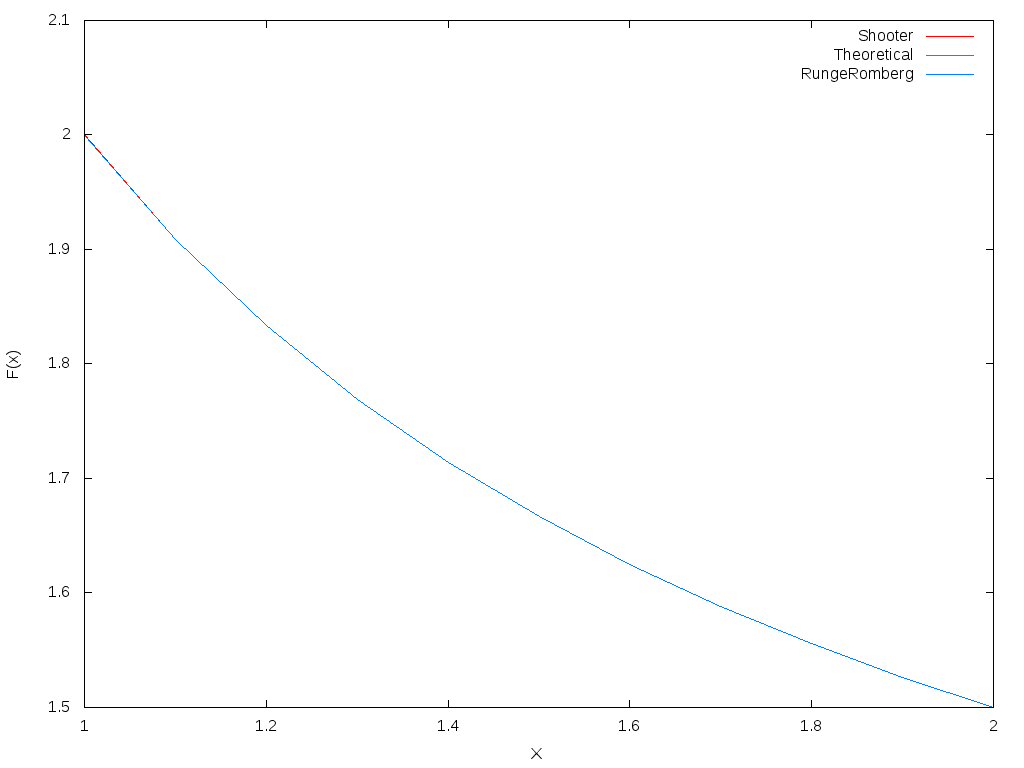
\includegraphics[scale=0.5]{images/graphic4_2Shooter.png}\\
\end{center}
\pagebreak
\begin{center}
\textbf{Рис. 2:} Метод конечных разностей\\
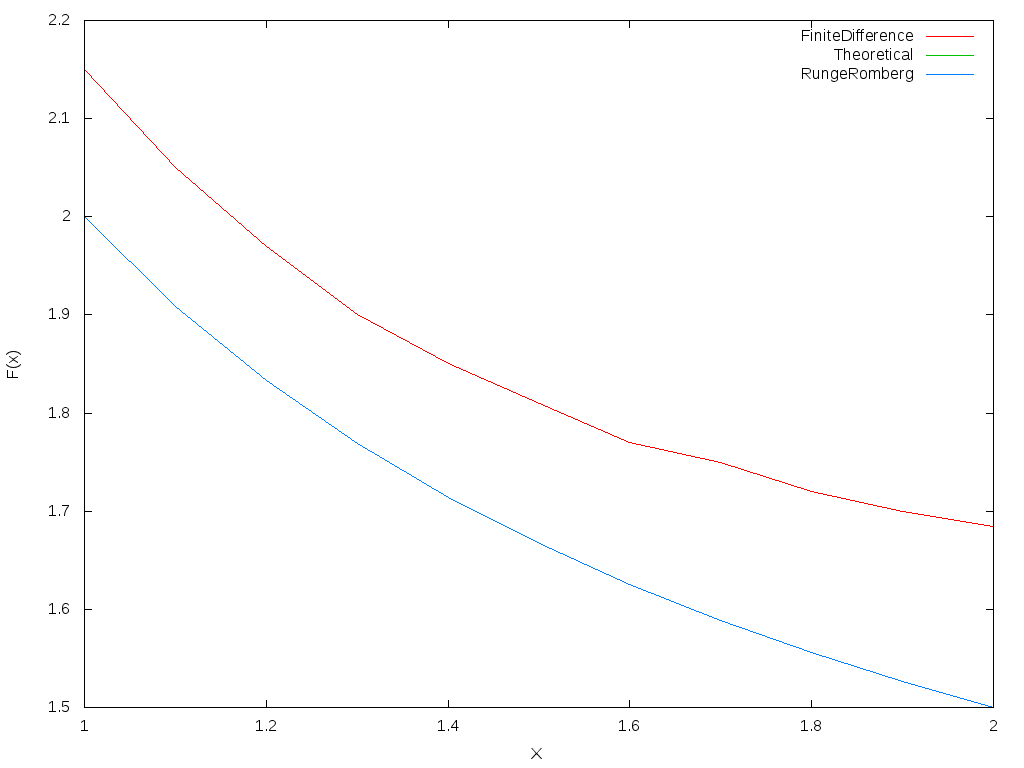
\includegraphics[scale=0.5]{images/graphic4_2FiniteDifference.png}\\
\end{center}

\pagebreak
